\section{Additional Performance Results and Throughput Breakdown}
\label{app:perf}
\label{app:perf-harness}

\sys{}' gains over the reference implementations all share one mechanism: \sys{}' state representations bound per-op cost by the spec, while the references' per-op cost grows with workload size. \cref{app:perf-curves} measures this on all five \sys{} suite specs with cluster-runnable implementations (RYW, MR, MW, RYW+MW, \sys{} suite CC), shows Chapar CC at the top of the figure for comparison, and adds an illustrative LCC row (labeled causal consistency: each client subscribes to a set of topic labels and only sees causality enforced on those). Across the \sys{} suite, throughput tracks consistency strength (RYW $>$ MW $>$ RYW+MW $>$ MR $>$ LCC $>$ \sys{} suite CC at put $=50\%$) because stricter specs require more checking work per operation. Chapar CC and \sys{} suite CC are both causal-consistency variants but their reference implementations are designed differently (Chapar's reads one position out of a flat list of per-write dependencies, while \sys{} suite's compares an entire per-client clock vector and atomically updates the writer's slot on every Put), so the two CC rows show different per-op work at the same correctness level. \cref{app:perf-cc,app:perf-mr} decompose the gap on Chapar CC and Monotonic Reads.

\paragraph{Setup details (extending \cref{sec:eval-setup}).}
Cluster zone: \texttt{us-central1-f}. Each VM is an \texttt{e2-standard-2} (2 vCPU, 8\,GB RAM) on Debian 12. Toolchain: OCaml 4.13.1 (dune 3.10) and \coq 8.18.0. Throughput is the sum across the $\text{NW}=4$ workers of $N / t_w$, where $t_w$ is each worker's wall-clock time and $N$ is its ops count, taking the median over three runs per cell; the put-rate sweep uses $N=1000$ (4{,}000 cluster ops total per run) and the scaling sweep varies $N \in \{1{,}000, 2{,}000, 5{,}000, 20{,}000\}$. Per-operation latency is bracketed inside the runtime around \texttt{put\_method}/\texttt{get\_method} and merged across workers; p99 is the 99th percentile of the pooled per-op latency distribution. Peak memory is the worker maximum of \texttt{Maximum resident set size} from \texttt{/usr/bin/time -v}, taking the median over three runs. Workload parameters: $\texttt{key\_range}=50$, $\texttt{val\_range}=100{,}000$, fixed seed $42$. The cluster uses a Chapar-style UDP runtime (\texttt{runtime\_doctex.ml}) adapted to the seven-method doctex \texttt{AlgDef} interface; we patched a socket bug for OCaml 4.13 / Debian 12.

\subsection{Per-protocol curves: all five \sys{} suite specs}
\label{app:perf-curves}


\paragraph{Result.}
Read-then-write specs cause the reference to exceed our $180$\,s wall-clock cap at every put rate measured: in \cref{fig:eval-perf-appendix} the reference's MW and RYW+MW rows show red $\times$ at every cell, with no measurable throughput. \sys{} runs cleanly throughout: $152$ kops/s on MW and $139$ kops/s on RYW+MW at put $=60\%$. The mechanism is a closure chain: the reference stores per-replica state as a function from key to value (a function-as-map); after extraction to OCaml, each prior \texttt{Put} adds a nested closure that a \texttt{Get} must unwrap. The read-then-write check re-evaluates this chain on every \texttt{Put}; combined with UDP packet reordering and the protocol's no-retry compare-and-swap, throughput collapses to zero. RYW has no read-then-write check, so its reference is competitive with \sys{} across the put-rate sweep: within roughly $20\%$ in either direction depending on workload mix, with \sys{} winning at low put rate (pct$=20$) and the reference faster at high put rate (pct$=60$--$70$). The reversal is a per-Put cost trade: \sys{}' assoc-list rewrites its spine on every \texttt{Put} ($O(K)$ cell allocations, $K$ = unique keys touched), while the reference's function-as-map prepends a single closure layer per \texttt{Put} ($O(1)$ heap cell). At low put rate the assoc-list's $O(K)$ \texttt{Get} lookup beats the reference's closure-chain walk; at high put rate the per-\texttt{Put} allocation cost dominates. MR shows the same chain-walk cost on \texttt{Get} (per-layer slope quantified in \cref{app:perf-mr}); \sys{} suite CC follows the same mechanism with \sys{}' balanced-tree store keeping Get logarithmic in distinct keys. Memory: \sys{}' assoc-list pays $0.1$--$1.0$ MB more on RYW (per-entry overhead) and runs in the same $5$--$6$ MB envelope as the reference on the other specs where the reference completes; on MW and RYW+MW the reference produces no memory measurement (it never completes a run). All memory traces are at $N=1{,}000$ ops/worker; \sys{} suite CC's vector-clock state is $O(\text{\#clients})$, so its trace is flat across the put-rate sweep at this workload size. At substantially larger $N$ or more clients, the message-bus and per-cell deps would push memory upward. The rightmost column (throughput vs $N$ at put $=50\%$) confirms the mechanism on every spec: the reference's throughput drops as $N$ grows because each new \texttt{Put} extends the chain, while \sys{}' assoc-list and balanced-tree structures keep throughput approximately flat. Across the put-rate sweep, both implementations' throughput falls and p99 latency rises as put-rate increases because each \texttt{Put} is broadcast to every replica, so more writes mean more in-flight messages and longer per-op queue waits.

\paragraph{Course correction on MW.}
Without performance feedback, \sys{} ships the first verifying design: a balanced-tree store. With performance feedback, the agent runs both candidates in its microbench harness and converges on the assoc-list, which the cluster benchmark harness confirms at $152$k ops/s at put $=60\%$ (\cref{fig:eval-perf-appendix}). Performance feedback changes the search policy, not the correctness criterion; both candidates are verified \sys{} suite refinements.

\subsection{Throughput breakdown: Chapar CC}
\label{app:perf-cc}

\begin{figure*}[t]
\centering
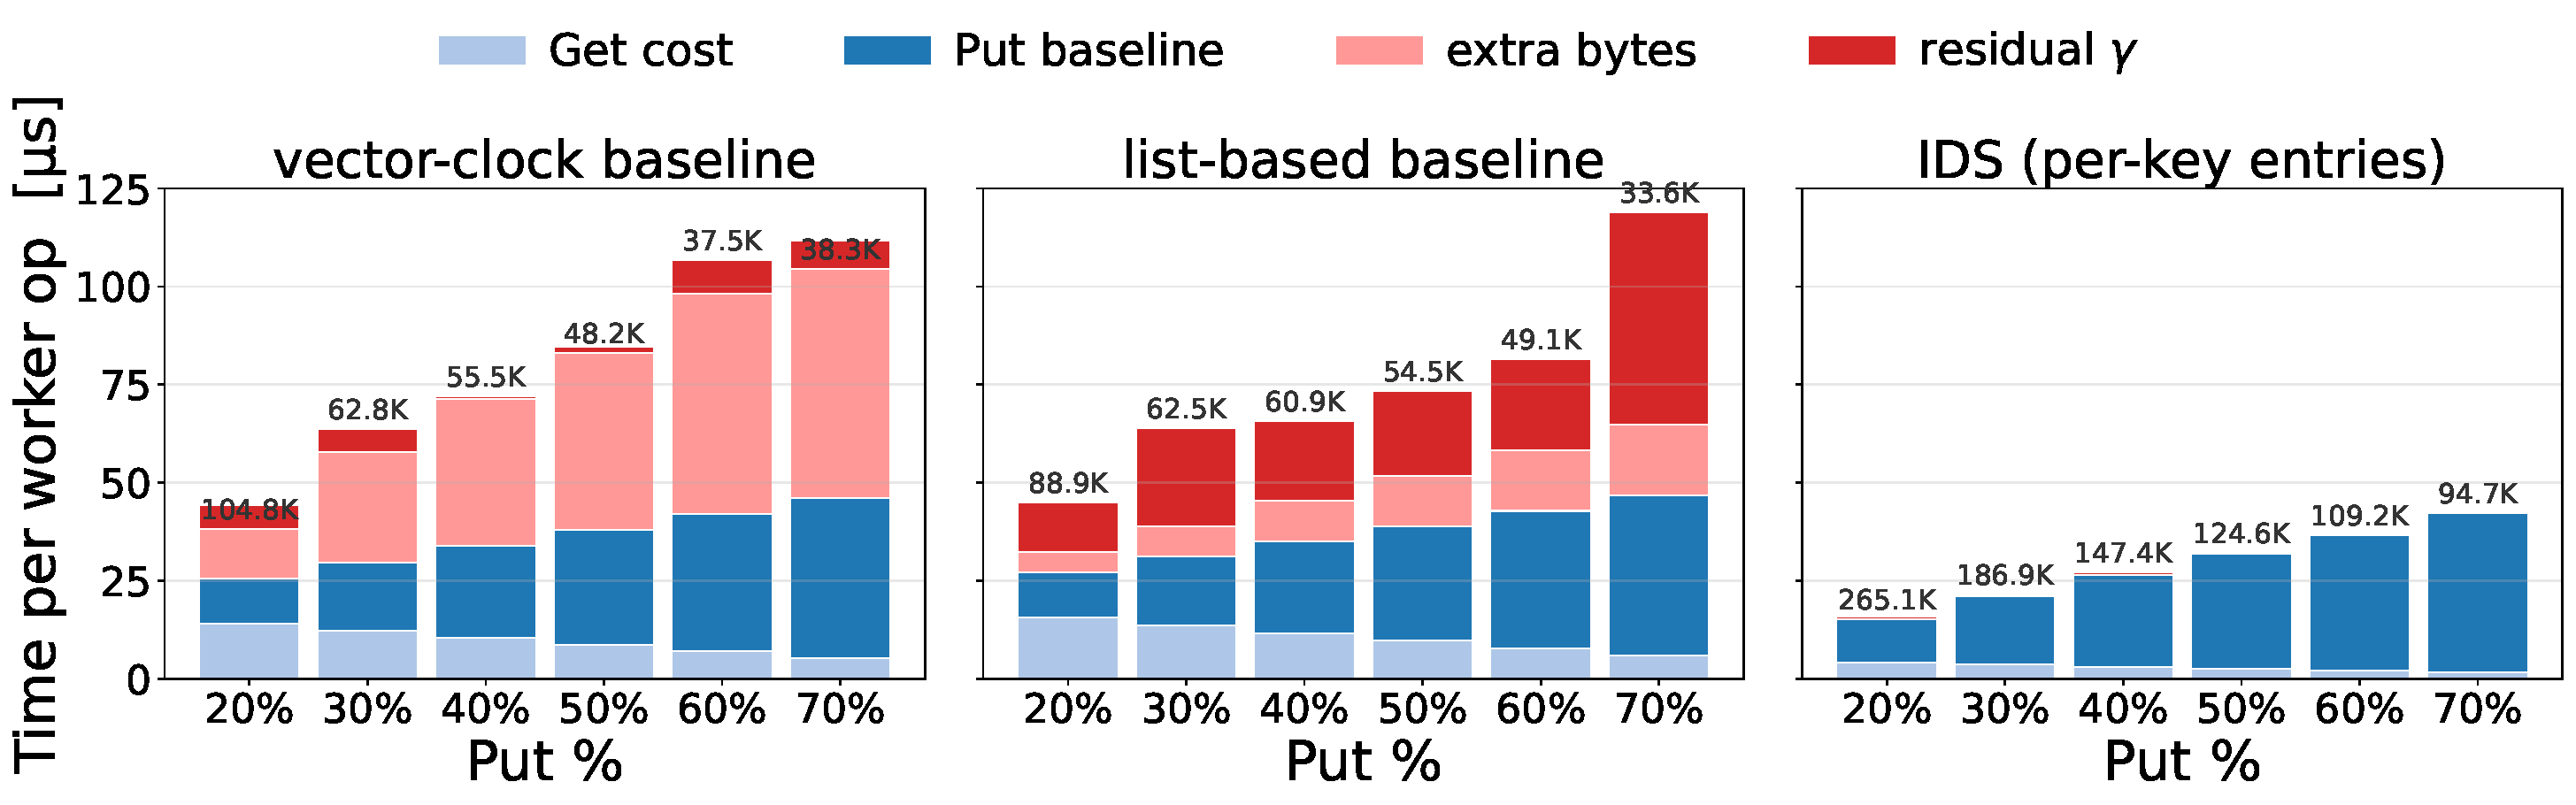
\includegraphics[width=\linewidth]{figures/figure_chapar_decomp.pdf}
\caption{Per-component decomposition of Chapar's two published baselines (vector-clock, list-based) and \sys{}' Chapar implementation (per-key store entries, used here as internal pivot). Bar height equals $4 / \text{(published cluster throughput)}$ in $\mu$s per worker op. Each bar splits into local Get cost, the per-key-entries Put baseline (same for all), per-algorithm extra wire bytes, and a per-algorithm residual $\gamma$. Segments sum to the published value at every cell by construction.}
\label{fig:chapar-decomp}
\end{figure*}

\paragraph{Setup.}
We attribute each algorithm's per-op time to four pieces: its Get cost (varies by algorithm), a shared Put baseline (per-key entries: $58.4\,\mu$s, the smallest of the three), a wire-bytes term proportional to extra bytes per Put ($\beta = 18\,\mu$s per byte, fit from vector-clock vs per-key entries), and a CPU residual $\gamma$ that captures whatever the wire-bytes term does not explain. Marshaled bytes per Put on the cluster: $44.81$ (vector-clock), $41.05$ (list-based), $39.62$ (per-key entries).

\paragraph{Result.}
Vector-clock loses on wire bytes; list-based loses on CPU. \textbf{Vector-clock} ships $+5.2$ bytes per Put over per-key entries, mapping to $+47\,\mu$s of per-op work at put $=50\%$; the residual $\gamma$ is $-1.75\,\mu$s, well below the bytes term. Almost the entire gap is wire bytes. \textbf{List-based} ships only $+1.4$ extra bytes per Put on average, yet $\gamma = +21.6\,\mu$s at put $=50\%$. The list-based replica stores the full history of delivered messages; receivers walk this list on every delivery (causality check), and \texttt{Get} walks it again to find the most-recent value for the requested key. Vector-clock and per-key entries do constant-time element-wise lookups.

\subsection{Throughput breakdown: Monotonic Reads}
\label{app:perf-mr}

\begin{figure*}[t]
\centering
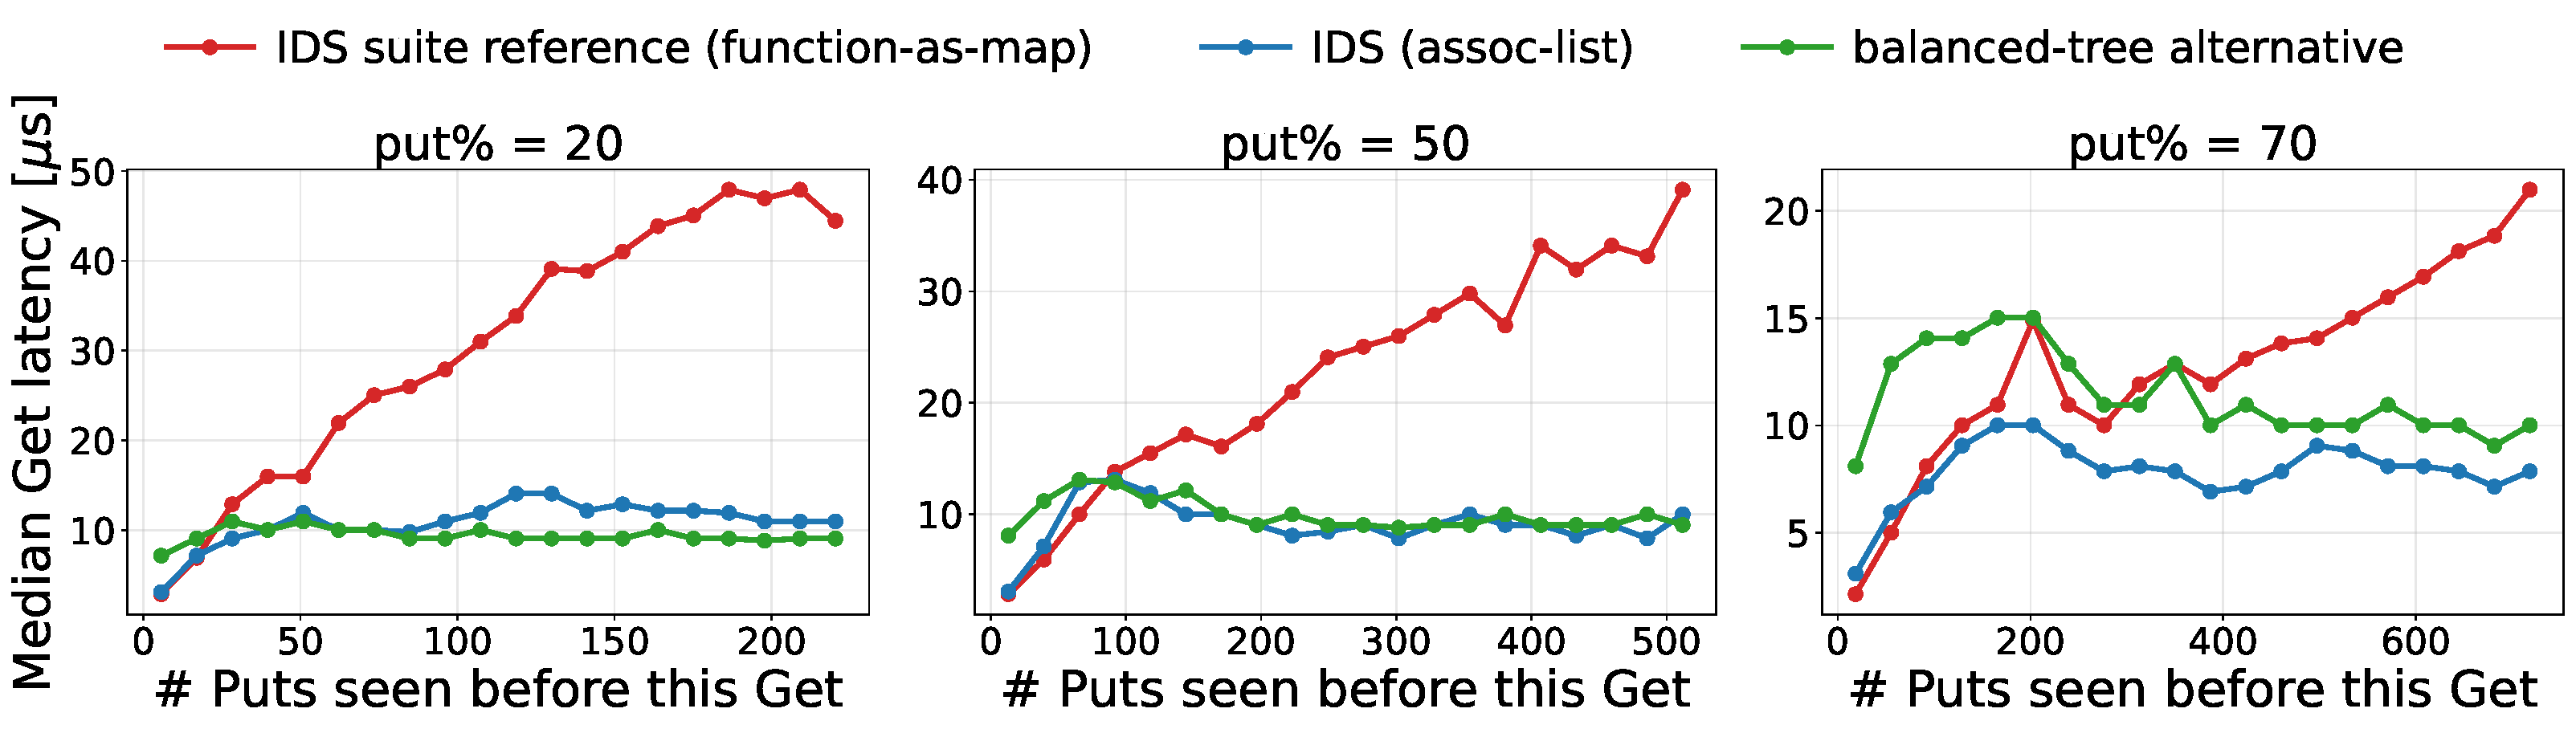
\includegraphics[width=\linewidth]{figures/figure_mr_get_vs_depth.pdf}
\caption{\texttt{Get} latency vs.\ closure depth (number of \texttt{Put}s preceding each \texttt{Get} in the same worker trace) for the three Monotonic Reads implementations at three put rates. The \sys{} suite reference's \texttt{Get} latency grows linearly with depth (slope $0.21\,\mu$s per closure layer at put $=20\%$, $R^2 = 0.95$). \sys{}' assoc-list slope is an order of magnitude smaller; the balanced-tree variant's slope is within statistical noise at every put rate.}
\label{fig:mr-depth}
\end{figure*}

\paragraph{Setup.}
Three MR implementations on the same runtime and identical wire format ($92.83$ B per \texttt{Put} on average): the \sys{} suite reference (function-as-map), \sys{} (assoc-list), and a balanced-tree alternative. Throughput differences are CPU-side. The balanced tree is a control: it tests whether \sys{}' win comes from the assoc-list specifically or from any structure that does not walk a closure chain on \texttt{Get}.

\paragraph{Where the cost lands.}
The reference pays on \texttt{Get}; the refinements pay on \texttt{Put}. At put $=50\%$:
\begin{center}
\begin{tabular}{lrr}
\toprule
implementation & $T_{\mathrm{get}}$ ($\mu$s) & $T_{\mathrm{put}}$ ($\mu$s) \\
\midrule
\sys{} suite reference (function-as-map) & $24.83$ & $15.40$ \\
\sys{} (assoc-list)                & $10.81$ & $16.81$ \\
balanced-tree alternative          & $11.40$ & $21.12$ \\
\bottomrule
\end{tabular}
\end{center}
Regressing \texttt{Get} latency against closure depth (number of \texttt{Put}s preceding a \texttt{Get} in the same worker trace) confirms the reference's chain walk: slope $0.21\,\mu$s/layer at put $=20\%$ ($R^2 = 0.95$, \cref{fig:mr-depth}). Both refinements stay flat across every put rate measured ($|\text{slope}| < 0.025\,\mu$s/layer): bounded data structure, no chain to walk. The balanced tree's extra Put cost comes from rebalance.

\paragraph{N-scaling at put $=50\%$.}
The reference's throughput drops as ops-per-worker $N$ grows; \sys{} stays nearly flat:
\begin{center}
\begin{tabular}{lrrrr}
\toprule
$N$ & $1{,}000$ & $2{,}000$ & $5{,}000$ & $20{,}000$ \\
\midrule
\sys{} suite reference (function-as-map) & $108{,}000$ & $100{,}000$ & $90{,}000$ & $80{,}000$ \\
\sys{} (assoc-list)                & $130{,}000$ & $124{,}000$ & $117{,}000$ & $112{,}000$ \\
\bottomrule
\end{tabular}
\end{center}
At $N=1{,}000$ \sys{} is $1.20\times$ faster; at $N=20{,}000$ the gap widens to $1.40\times$. Throughput drop from $N=1{,}000$ to $N=20{,}000$: reference $1.35\times$, \sys{} $1.16\times$. The reference's per-\texttt{Get} closure walk grows linearly with prior \texttt{Put}s, so its per-op cost rises with $N$; the assoc-list's lookup is bounded by the number of distinct keys in the workload (50 here), so its per-op cost is $N$-independent and only message-bus pressure causes the mild decline.


\newpage


\begin{figure*}[t]
\centering
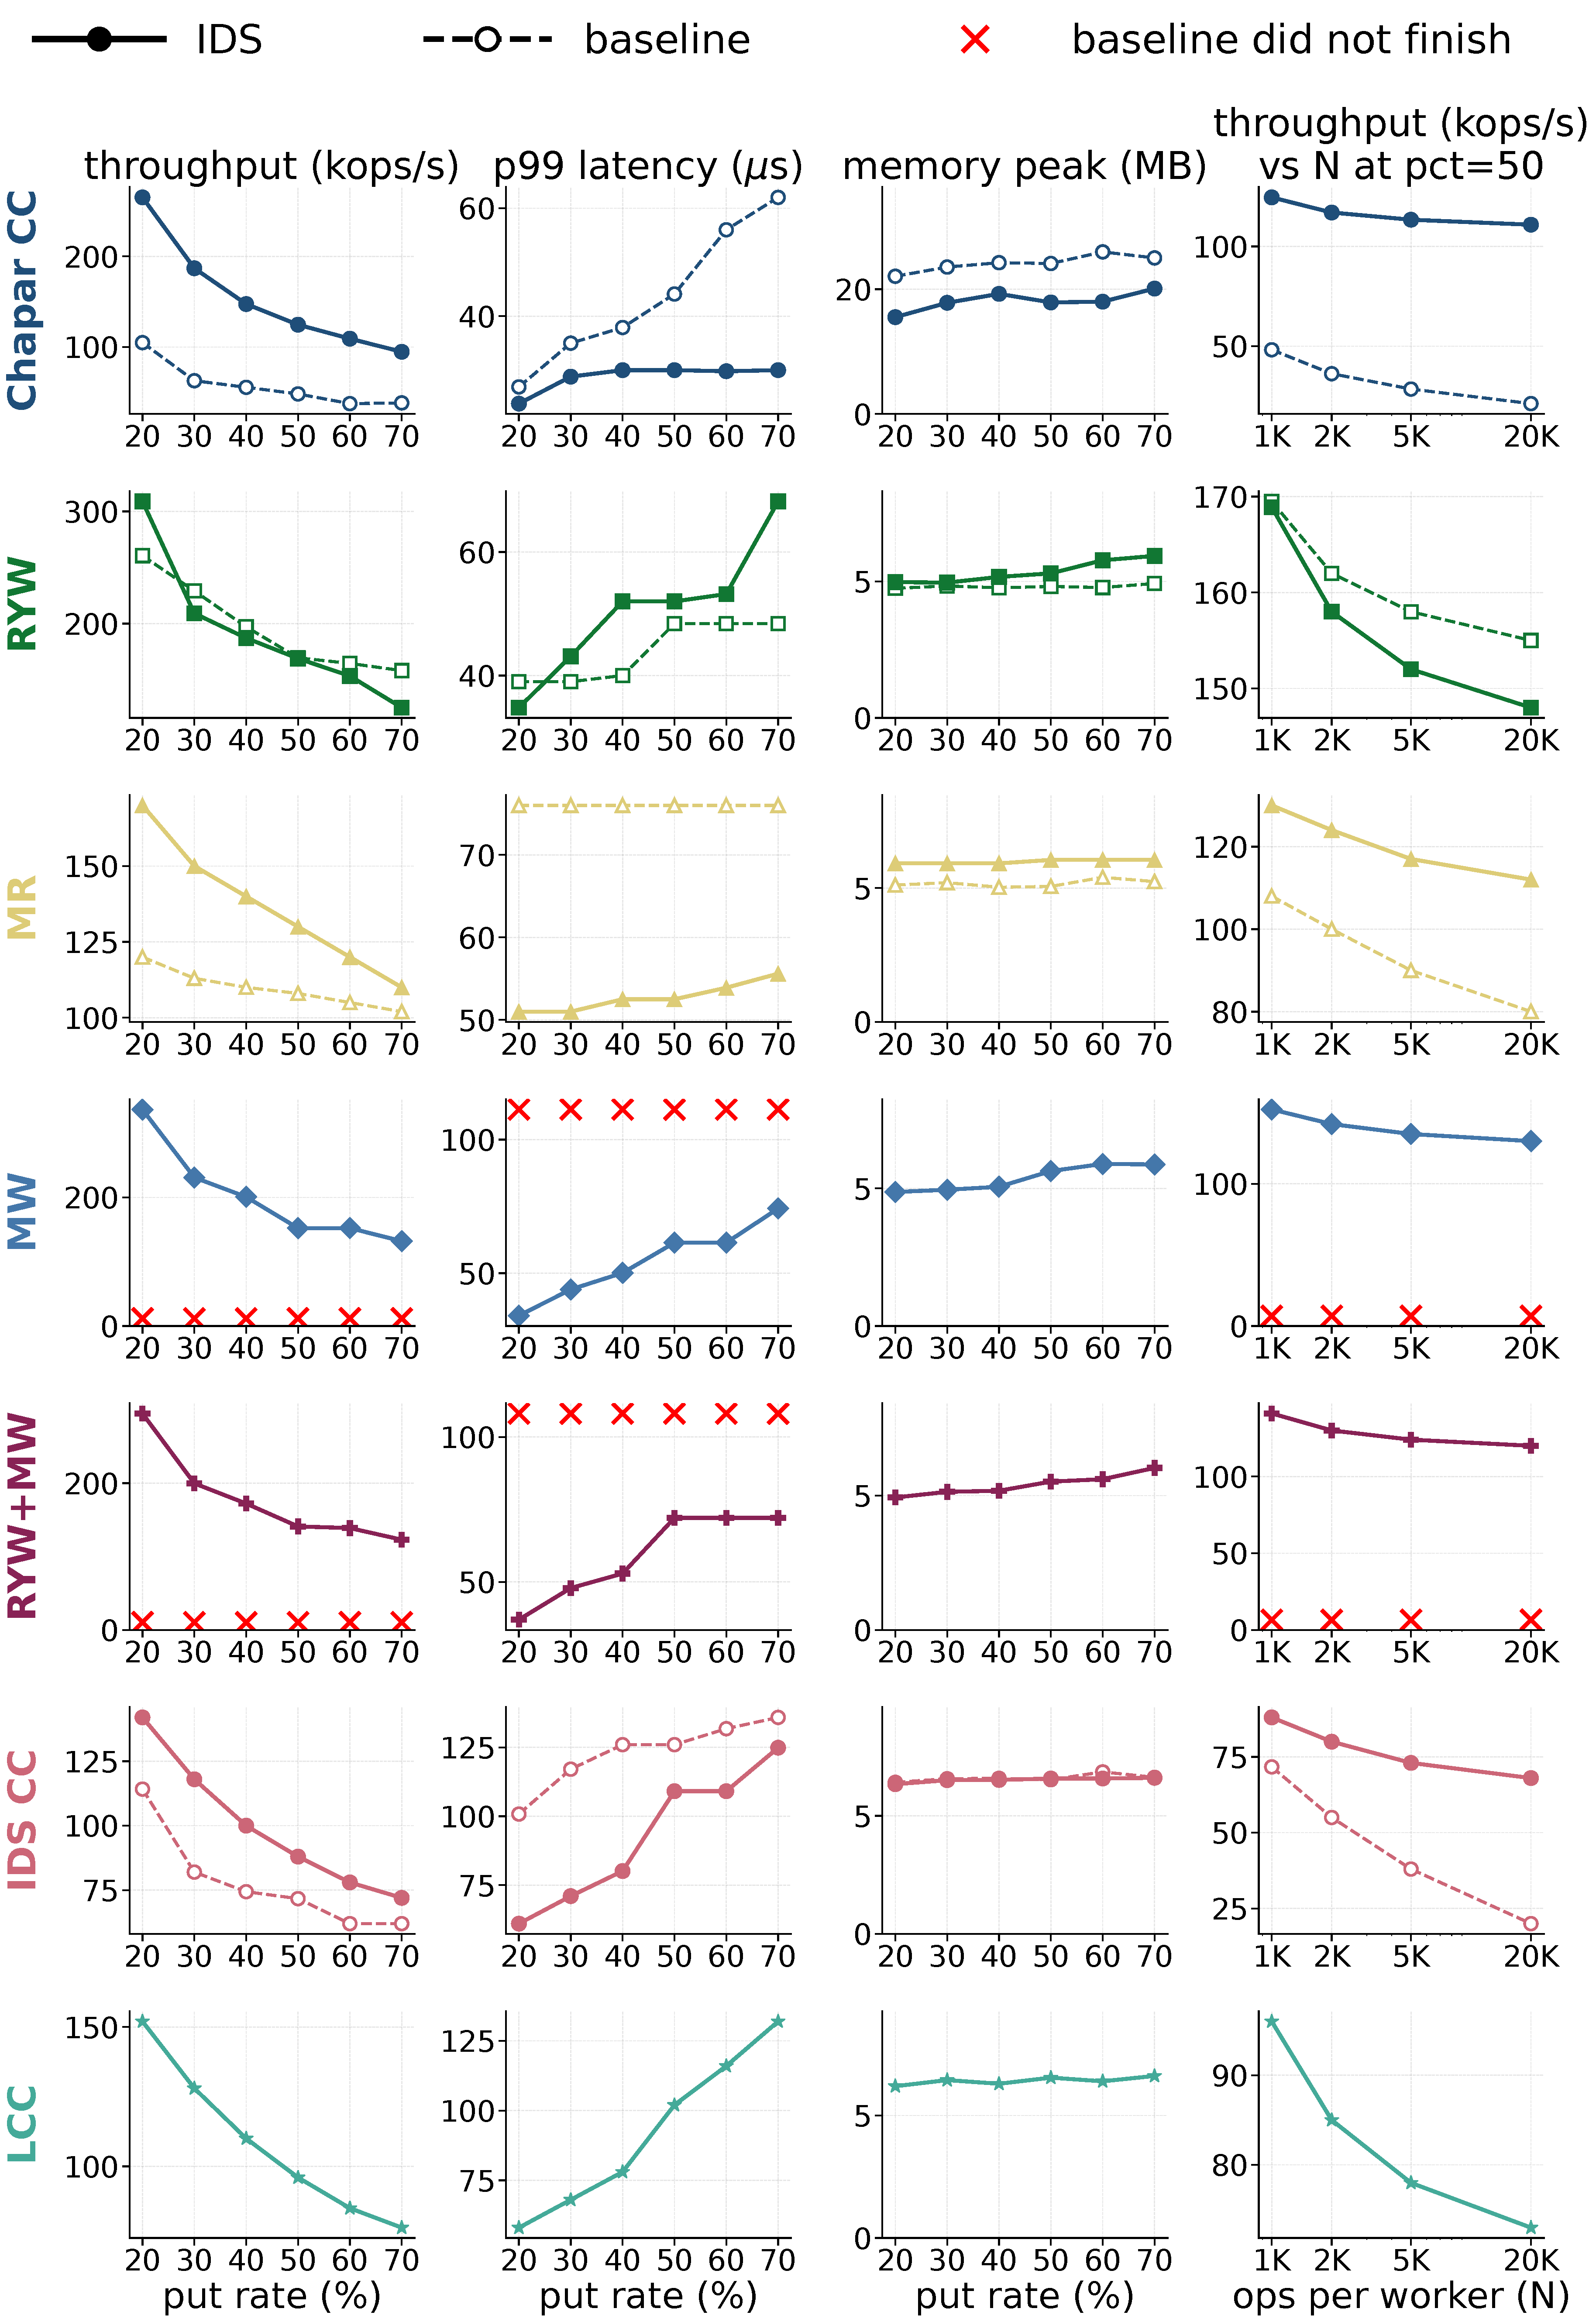
\includegraphics[width=\linewidth]{figures/eval_perf_appendix.pdf}
\caption{Per-protocol performance. Top row is Chapar CC (Chapar paper protocol) shown for comparison; the next five rows are the \sys{} suite specs (RYW, MR, MW, RYW+MW, \sys{} suite CC); the bottom LCC row is a single-line illustrative trajectory of labeled causal consistency. Columns: throughput (kops/s), p99 latency ($\mu$s), memory peak (MB), and throughput vs ops-per-worker $N$ at put $=50\%$. Per-protocol $y$-axes are dedicated so each row's range is visible. Solid $=$ \sys{}; dashed $=$ reference (function-as-map). Red $\times$ marks runs that hit the $180$\,s wall-clock cap; on MW and RYW+MW the reference times out at every put rate (the reference's read-then-write check on a function-as-map is the cause; see below).}
\label{fig:eval-perf-appendix}
\end{figure*}
